%%%%%%%%%%%%%%%%%%%%%%%%%%%%%%%%%%%%%%%%%
% Lachaise Assignment
% LaTeX Template
% Version 1.0 (26/6/2018)
%
% This template originates from:
% http://www.LaTeXTemplates.com
%
% Authors:
% Marion Lachaise & François Févotte
% Vel (vel@LaTeXTemplates.com)
%
% License:
% CC BY-NC-SA 3.0 (http://creativecommons.org/licenses/by-nc-sa/3.0/)
% 
%%%%%%%%%%%%%%%%%%%%%%%%%%%%%%%%%%%%%%%%%

%----------------------------------------------------------------------------------------
%	PACKAGES AND OTHER DOCUMENT CONFIGURATIONS
%----------------------------------------------------------------------------------------

\documentclass{article}

%%%%%%%%%%%%%%%%%%%%%%%%%%%%%%%%%%%%%%%%%
% Lachaise Assignment
% Structure Specification File
% Version 1.0 (26/6/2018)
%
% This template originates from:
% http://www.LaTeXTemplates.com
%
% Authors:
% Marion Lachaise & François Févotte
% Vel (vel@LaTeXTemplates.com)
%
% License:
% CC BY-NC-SA 3.0 (http://creativecommons.org/licenses/by-nc-sa/3.0/)
% 
%%%%%%%%%%%%%%%%%%%%%%%%%%%%%%%%%%%%%%%%%

%----------------------------------------------------------------------------------------
%	PACKAGES AND OTHER DOCUMENT CONFIGURATIONS
%----------------------------------------------------------------------------------------

\usepackage{keystroke} % https://ctan.crest.fr/tex-archive/macros/latex/contrib/keystroke/key-test.pdf

\usepackage{amsmath,amsfonts,stmaryrd,amssymb} % Math packages

\usepackage{minted} % Code

\usepackage{enumerate} % Custom item numbers for enumerations

\usepackage{algpseudocode} % Pseudo-code package

\usepackage[ruled]{algorithm2e} % Algorithms
\SetKwInput{KwIn}{Data}
\SetKwInput{KwOut}{Output}





\usepackage[framemethod=tikz]{mdframed} % Allows defining custom boxed/framed environments

\usepackage{dirtree} % Arbre 

\usepackage{listings} % File listings, with syntax highlighting

\usepackage{xcolor}

\usepackage{graphicx}

\usepackage{hyperref}

\lstset{
	basicstyle=\ttfamily, % Typeset listings in monospace font
}

%----------------------------------------------------------------------------------------
%	DOCUMENT MARGINS
%----------------------------------------------------------------------------------------

\usepackage{geometry} % Required for adjusting page dimensions and margins

\geometry{
	paper=a4paper, % Paper size, change to letterpaper for US letter size
	top=2.5cm, % Top margin
	bottom=3cm, % Bottom margin
	left=2.5cm, % Left margin
	right=2.5cm, % Right margin
	headheight=14pt, % Header height
	footskip=1.5cm, % Space from the bottom margin to the baseline of the footer
	headsep=1.2cm, % Space from the top margin to the baseline of the header
	%showframe, % Uncomment to show how the type block is set on the page
}

%----------------------------------------------------------------------------------------
%	FONTS
%----------------------------------------------------------------------------------------

\usepackage[utf8]{inputenc} % Required for inputting international characters
\usepackage[T1]{fontenc} % Output font encoding for international characters

\usepackage{XCharter} % Use the XCharter fonts

%----------------------------------------------------------------------------------------
%	COMMAND LINE ENVIRONMENT
%----------------------------------------------------------------------------------------

% Usage:
% \begin{commandline}
%	\begin{verbatim}
%		$ ls
%		
%		Applications	Desktop	...
%	\end{verbatim}
% \end{commandline}

\mdfdefinestyle{commandline}{
	leftmargin=10pt,
	rightmargin=10pt,
	innerleftmargin=15pt,
	middlelinecolor=black!50!white,
	middlelinewidth=2pt,
	frametitlerule=false,
	backgroundcolor=black!5!white,
	frametitle={Command Line},
	frametitlefont={\normalfont\sffamily\color{white}\hspace{-1em}},
	frametitlebackgroundcolor=black!50!white,
	nobreak,
}

% Define a custom environment for command-line snapshots
\newenvironment{commandline}{
	\medskip
	\begin{mdframed}[style=commandline]
}{
	\end{mdframed}
	\medskip
}

%----------------------------------------------------------------------------------------
%	FILE CONTENTS ENVIRONMENT
%----------------------------------------------------------------------------------------

% Usage:
% \begin{file}[optional filename, defaults to "File"]
%	File contents, for example, with a listings environment
% \end{file}

\mdfdefinestyle{file}{
	innertopmargin=1.6\baselineskip,
	innerbottommargin=0.8\baselineskip,
	topline=false, bottomline=false,
	leftline=false, rightline=false,
	leftmargin=2cm,
	rightmargin=2cm,
	singleextra={%
		\draw[fill=black!10!white](P)++(0,-1.2em)rectangle(P-|O);
		\node[anchor=north west]
		at(P-|O){\ttfamily\mdfilename};
		%
		\def\l{3em}
		\draw(O-|P)++(-\l,0)--++(\l,\l)--(P)--(P-|O)--(O)--cycle;
		\draw(O-|P)++(-\l,0)--++(0,\l)--++(\l,0);
	},
	nobreak,
}

% Define a custom environment for file contents
\newenvironment{file}[1][File]{ % Set the default filename to "File"
	\medskip
	\newcommand{\mdfilename}{#1}
	\begin{mdframed}[style=file]
}{
	\end{mdframed}
	\medskip
}

%----------------------------------------------------------------------------------------
%	NUMBERED QUESTIONS ENVIRONMENT
%----------------------------------------------------------------------------------------

% Usage:
% \begin{question}[optional title]
%	Question contents
% \end{question}

\mdfdefinestyle{question}{
	innertopmargin=1.2\baselineskip,
	innerbottommargin=0.8\baselineskip,
	roundcorner=5pt,
	nobreak,
	singleextra={%
		\draw(P-|O)node[xshift=1em,anchor=west,fill=white,draw,rounded corners=5pt]{%
		Question \theQuestion\questionTitle};
	},
}

\newcounter{Question} % Stores the current question number that gets iterated with each new question

% Define a custom environment for numbered questions
\newenvironment{question}[1][\unskip]{
	\bigskip
	\stepcounter{Question}
	\newcommand{\questionTitle}{~#1}
	\begin{mdframed}[style=question]
}{
	\end{mdframed}
	\medskip
}

%----------------------------------------------------------------------------------------
%	WARNING TEXT ENVIRONMENT
%----------------------------------------------------------------------------------------

% Usage:
% \begin{warn}[optional title, defaults to "Warning:"]
%	Contents
% \end{warn}

\mdfdefinestyle{warning}{
	topline=false, bottomline=false,
	leftline=false, rightline=false,
	nobreak,
	singleextra={%
		\draw(P-|O)++(-0.5em,0)node(tmp1){};
		\draw(P-|O)++(0.5em,0)node(tmp2){};
		\fill[black,rotate around={45:(P-|O)}](tmp1)rectangle(tmp2);
		\node at(P-|O){\color{white}\scriptsize\bf !};
		\draw[very thick](P-|O)++(0,-1em)--(O);%--(O-|P);
	}
}

% Define a custom environment for warning text
\newenvironment{warn}[1][Warning:]{ % Set the default warning to "Warning:"
	\medskip
	\begin{mdframed}[style=warning]
		\noindent{\textbf{#1}}
}{
	\end{mdframed}
}

%----------------------------------------------------------------------------------------
%	INFORMATION ENVIRONMENT
%----------------------------------------------------------------------------------------

% Usage:
% \begin{info}[optional title, defaults to "Info:"]
% 	contents
% 	\end{info}

\mdfdefinestyle{info}{%
	topline=false, bottomline=false,
	leftline=false, rightline=false,
	nobreak,
	singleextra={%
		\fill[black](P-|O)circle[radius=0.4em];
		\node at(P-|O){\color{white}\scriptsize\bf i};
		\draw[very thick](P-|O)++(0,-0.8em)--(O);%--(O-|P);
	}
}

% Define a custom environment for information
\newenvironment{info}[1][Info:]{ % Set the default title to "Info:"
	\medskip
	\begin{mdframed}[style=info]
		\noindent{\textbf{#1}}
}{
	\end{mdframed}
}


%----------------------------------------------------------------------------------------
%	EQUATION
%----------------------------------------------------------------------------------------

\newcommand{\equabezier}{
	\begin{displaymath}
		P(t) = P_0(1-t)^3+3P_1t(1-t)^2+3P_2t^2(1-t)+P_3t^3	
	\end{displaymath}
} % Include the file specifying the document structure and custom commands

%----------------------------------------------------------------------------------------
%	ASSIGNMENT INFORMATION
%----------------------------------------------------------------------------------------

\title{Mathématiques pour l'Informatique : Compte Rendu} % Title of the assignment
\author{Valentin VERSTRACTE \& Evan PETIT}

\date{L3 --- Jean-Luc BARIL --- \today} % University, school and/or department name(s) and a date



%----------------------------------------------------------------------------------------

\begin{document}

\maketitle % Print the title

%----------------------------------------------------------------------------------------
%	Table des matières
%----------------------------------------------------------------------------------------
\bigskip
\bigskip
\renewcommand{\contentsname}{Table des matières}
\tableofcontents
\vspace{75pt}

%----------------------------------------------------------------------------------------
% 
%----------------------------------------------------------------------------------------
\newpage
\section{Introduction} 

Ce rapport concerne le rendu du projet de Mathématiques pour l'informatique. Le projet a été intégralement réalisé en collaboration sur GitHub, en langage C++ pour l'implémentation des algorithmes, et en \LaTeX pour le compte-rendu.\\~\\
Sommaire des fonctionnalités implémentées :


\begin{description}
	\item [Transformée de Fourier discrète 1D \& 2D] Implémentation de la transformée discrète directe et inverse depuis la formule mathématique 
	\item [Transformée de Fourier rapide 1D \& 2D] Implémentation de la transformée rapide avec l'algorithme de Cooley-Tukey
	\item [Séquence de tests] Vérification des résultats obtenus 
\end{description}
\newpage
\section{Transformée de Fourier discrète}



\subsection{Transformée de Fourier 1D directe et inverse}

\subsubsection{Formule}
On rappelle la formule, où \textbf{g(x)} est le signal original, et \textbf{$\widehat{\textbf{g}}$(x)} est son calcul par la TFD. La transformée de Fourier directe permet d'obtenir $\widehat{g}$(x) depuis g(x).

\begin{equation}
		\widehat{g}(k) = \sum_{x = 0}^{N-1}g(x) exp(\frac{-2i\pi kx}{N}) \qquad pour \qquad 0 \leq k < N
\end{equation}

\noindent L'inverse permet... L'inverse. On remarque l'introduction d'une multiplication d'un facteur -1 dans l'exponentielle

\begin{equation}
	g(k) = \sum_{x = 0}^{N-1}\widehat{g}(x) exp(\frac{2i\pi kx}{N}) \qquad pour \qquad 0 \leq k < N
\end{equation}


\noindent L'algorithme équivalent peut être implémenté de façon brutale. On a besoin de deux boucles : Une pour calculer le produit à l'intérieur de la somme pour les valeurs de k allant de 0 à N-1, et une pour sommer tous les résultats obtenus pour x allant de 0 à N-1. Modulo un facteur -1 pour obtenir la transformée inverse.


\begin{algorithm}
	\caption{Transformée discrète 1D directe}\label{alg:cap}
	\KwIn{$g[N]$ : Vecteur 1D complexe}
	\KwOut{$G[N]$ : Vecteur 1D complexe}
	\Begin{
		\For{$k \gets 0 .. N-1$}
		{   
			\For{$x \gets 0 .. N-1$}
			{
				$G[k] \gets G[k] + g[x] * $(exponentielle complexe en fonction de k et x)
			}
		}		
	}		
\end{algorithm}

Comme dit précédemment, la transformée inverse ne demande que l'introduction d'un facteur -1 dans le contenu de l'exponentielle, ainsi que de diviser chaque indice de vecteur par la taille totale du vecteur)

\subsubsection{Complexité}

La complexité de l'algorithme se déduit assez facilement. Soit \textbf{g} le vecteur passé en entrée, de taille \textbf{n}, et \textbf{k} un indice quelconque de g.
\begin{itemize}
	\item Pour calculer \textbf{g[k]} il faut calculer le produit de g[0] avec une exponentielle complexe, de même pour g[1], g[2], . . . , g[n-1] et faire la somme de tous ces produits. Le tableau est de taille n, on fait donc n produits ainsi qu'une addition (négligeable). On peut dire qu'on effectue \textbf{n} opérations élémentaires.
	\item Il faut répéter cette étape autant de fois qu'il y a d'indices dans le tableau. C'est à dire \textbf{n} fois.
	\item Au total on compte (à quelques constantes près) \textbf{n*n} opérations.
	La complexité finale est donc de l'ordre de O(n * n) = \textbf{O(n²)} 
\end{itemize}

\subsubsection{Diagramme}

On peut réaliser un simple diagramme pour représenter cet algorithme. Ici g[x] est le signal d'entrée (représenté par un vecteur 1D), et G[x] le vecteur en sortie. Ils sont de taille N.

\begin{figure}[!htb]
	\centering
	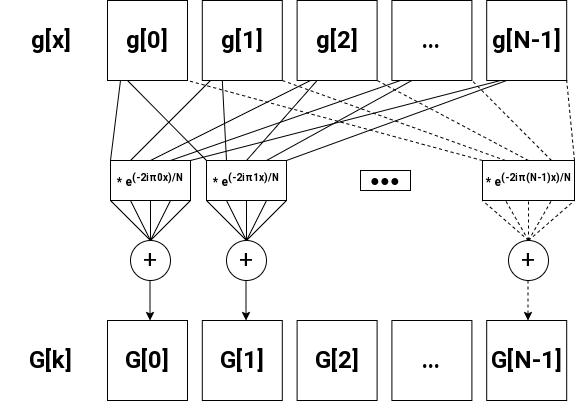
\includegraphics[height=8cm]{./assets/TFD1D.png}
	\caption{TFD 1D}
	\label{fig:TFD1D}
\end{figure}

\subsection{Transformée de Fourier 2D discrète}

La formule de la transformée de Fourier 2D discrète directe pour une matrice de taille N,M est la suivante

\begin{equation}
	\widehat{g}(k,j) = \sum_{x = 0}^{N-1}\sum_{y = 0}^{M-1}g(x,y) exp(-2i\pi(\frac{jx}{N}+\frac{ky}{M})) \quad pour \quad 0 \leq j < N\quad et \quad 0 \leq k < M
\end{equation}

Cette fois-ci on boucle sur 2 éléments de taille N (x et j), et 2 éléments de taille M (y et k). La complexité ne s'exprime plus en O(N²) mais en \textbf{O(N²M²)}. Si on introduit une matrice carrée de taille N,N cela signifie que la complexité est en \textbf{\textit{O($\textbf{N}^4$)}}. C'est gigantesque.\\

\noindent On admettra la propriété énonçant que la transformée de Fourier discrète directe (et indirecte) d'une matrice 2D consiste à effectuer la transformée de Fourier 1D des lignes, suivie de la transformée de Fourier 1D des colonnes.

\begin{figure}[!htb]
	\centering
	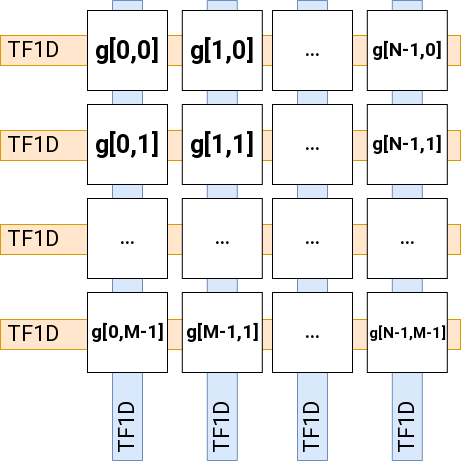
\includegraphics[height=7cm]{./assets/TFD2D.png}
	\caption{TFD 2D}
	\label{fig:TFD2D}
\end{figure}



\section{Transformée de Fourier rapide}

La transformée de Fourier directe présente un défaut majeur : Son absurde lenteur. On a vu que la transformée de Fourier discrète 1D possédait une complexité polynomiale (en temps O($N^2$)).\\
Si l'on considère un vecteur de taille $N$ avec $N = 2^{12} = 4096$, et la durée d'une opération élémentaire de $10ns$, alors le calcul de la transformée de Fourier de cette matrice prendrait $4096^2*10 = 167772160ns = 0.17s = \textbf{18\:minutes}$.\\
Pour un algorithme que l'on retrouve dans énormément de domaines - tant qu'il s'agit d'un pilier de l'informatique moderne - C'est beaucoup trop long.\\
On chercherait plutôt à se retrouver avec une complexité presque linéaire qu'on retrouve souvent en algorithmique, c'est à dire en temps $\textbf{O(n log(n))}$. Avec un tel algorithme, le temps de calcul pour une matrice avec $N = 2^{12}$, le temps de calcul chuterait à \textbf{491 520 ns}, une différence d'ordre de grandeur de $10^3$!\\~\\
Un algorithme permet cela, il s'agit de la transformée de Fourier rapide. Dans la suite sera présentée la version récursive de cet algorithme par les informaticiens \textbf{Cooley \& Tukey} - Elle a pour avantage d'être assez simple, élégante, et il s'agit de la première version de cet algorithme à être vastement employée. Ses désavantages principaux sont de ne pouvoir travailler qu'avec des vecteurs ayant une taille en puissances de deux - et de devoir se servir de la pile de récursion qui est assez limitée en fonction du langage de programmation.
Mais il s'agit d'une très bonne porte d'entrée pour la compréhension de la Transformée de Fourier rapide (la \textbf{FFT} pour \textbf{F}ast \textbf{F}ourier \textbf{T}ransform).\\

\noindent \textbf{Nous ne présenterons que la transformée rapide 1D} - En effet on a vu précédemment que la transformée 2D était la composée de deux transformée 1D.

\subsection{Principe de l'algorithme de Cooley-Tukey}

A l'instar du tri fusion ou du tri rapide, cet algorithme se base sur le principe \textit{Divide and Conquer}. \\
En \textbf{divisant} (divide) le vecteur de base en deux sous-vecteurs de taille inférieure N/2, diviser ces sous-vecteurs en sous-sous-vecteurs, etc... On peut traiter des vecteurs de taille 1. La transformée de Fourier discrète d'un vecteur de taille 1 étant excessivement simple à calculer, et alors il suffit juste de \textbf{recombiner} (conquer) ces vecteurs entre eux pour obtenir le résultat : Ce type de schéma se prête très fortement à la récursion - \textit{même si les algorithmes récents cherchent à l'éviter à cause de soucis de performance} - car on procède en problèmes de plus en plus petits.\\~\\
Cependant, comment choisir de quelle manière diviser ces vecteurs? Il est possible de manipuler légèrement la formule de la transformée de Fourier directe pour obtenir ce que l'on souhaite.

\subsection{Décomposition}

Soit la formule de la transformée de Fourier 1D. \textbf{g} est le vecteur donné en entrée \textbf{G} est le calcul de la FFT de ce même vecteur, de taille $\textbf{N} = 2^{n}$.

\begin{equation}
	G_{k} = \sum_{x = 0}^{N-1}g_{x} exp(\frac{-2i\pi kx}{N}) \qquad pour \qquad 0 \leq k < N
\end{equation}

\subsubsection{Indices pairs et impairs}

La manière la plus courante pour décomposer cette équation en somme de deux termes est de séparer les indices pairs et impairs : x devient alors 2p ou 2p+1 en fonction de sa \textbf{parité.} Puisque N est une puissance de 2, il est pair, donc les deux sous-sommes obtenues sont de même taille : \textbf{N/2}

\begin{equation}
	G_{k} = \underbrace{\sum_{p = 0}^{N/2-1}g_{2p} exp(\frac{-2i\pi k(2p)}{N})}_\text{Indices pairs} + \underbrace{\sum_{p = 0}^{N/2-1}g_{2p+1} exp(\frac{-2i\pi k(2p+1)}{N})}_\text{Indices impairs} \qquad pour \qquad 0 \leq k < N
\end{equation}

\newpage Un des premiers éléments clés de cet algorithme apparaît alors. Même si pour le moment, le contenu des deux sommes n'est pas le même, il est possible que les exponentielles complexes le soient! Dans la somme des indices impairs, il suffit de factoriser par une \textbf{constante obtenue depuis le (2p+1)} :

\begin{equation}
	G_{k} = \underbrace{\sum_{p = 0}^{N/2-1}g_{2p} exp(\frac{-2i\pi k(2p)}{N})}_\text{Indices pairs} + \underbrace{  \sum_{p = 0}^{N/2-1}g_{2p+1} exp(\frac{-2i\pi k(2p)}{N} + \overbrace{\frac{-2i\pi k*1}{N}}^\text{Constante} )  }_\text{Indices impairs} \quad pour \quad 0 \leq k < N
\end{equation}
\begin{equation}
	G_{k} = \underbrace{\sum_{p = 0}^{N/2-1}g_{2p} exp(\frac{-2i\pi kp}{N})}_\text{Indices pairs} + \underbrace{exp(\frac{-2i\pi k}{N/2})\sum_{p = 0}^{N/2-1}g_{2p+1} exp(\frac{-2i\pi k	p}{N/2})}_\text{Indices impairs} \quad pour \quad 0 \leq k < N
\end{equation}

On peut déjà remarquer que les deux sommes correspondent à la formule de deux transformées de Fourier. Si l'on appelle \textbf{P} la transformée de Fourier des indices \textbf{P}airs, et \textbf{I} la transformée de fourier des indices \textbf{I}mpairs, alors on a :

\begin{equation}
	G_{k} = \underbrace{\sum_{p = 0}^{N/2-1}g_{2p} exp(\frac{-2i\pi kp}{N/2})}_\text{Transformée de Fourier aux indices pairs : $P_{k}$} + exp(\frac{-2i\pi k}{N})\underbrace{\sum_{p = 0}^{N/2-1}g_{2p+1} exp(\frac{-2i\pi k	p}{N/2})}_\text{Transformée de Fourier aux indices impairs : $I_{k}$} \quad pour \quad 0 \leq k < N
\end{equation}
\begin{equation}
	G_{k} = P_{k} + \underbrace{exp(\frac{-2i\pi k}{N})}_\text{Constante} I_{k} \quad pour \quad 0 \leq k < N
\end{equation}

\subsubsection{Plage de valeurs de k}

Il reste une dernière épine dans le pied : La plage de valeurs de k. En effet, on calcule G pour k de 0 à N-1, mais il est possible de vérifier que cette équation reste la même pour \textbf{k de 0 à N/2 - 1} et pour \\\textbf{k + N/2 avec k de 0 à N/2 - 1} (l'union de ces deux intervalles étant bien k de 0 à N-1)\\~\\

\noindent\qquad \textbf{Cas de l'exponentielle contenue dans $I_{k}$ et $P_{k}$ , avec k de 0 à N/2-1}\\~\\
Remplaçons k par k+N/2 et essayons de supprimer le terme N/2. Pour cela servons nous de la forme trigonométrique pour jouer avec la périodicité des fonctions sin et cos :
\begin{equation}
	exp(\frac{-2i\pi (k+N/2)p}{N/2}) = cos(\frac{-2\pi (k+N/2)p}{N/2})+i\:sin(\frac{-2\pi (k+N/2)p}{N/2})
\end{equation}
On peut distribuer (k+N/2) et simplifier :
\begin{equation}
	exp(\frac{-2i\pi (k+N/2)p}{N/2}) = cos(\frac{-2\pi (N/2)p-2\pi k}{N/2})+i\:sin(\frac{-2\pi (N/2)p-2\pi k}{N/2})
\end{equation}
\begin{equation}
	exp(\frac{-2i\pi (k+N/2)p}{N/2}) = cos(-2\pi p+\frac{2\pi k}{N/2})+i\:sin(-2\pi p+\frac{2\pi k}{N/2})
\end{equation}
Or, les fonctions cosinus et sinus sont de période $2\pi$, de plus p est un entier. On peut donc se débarrasser des termes fraîchement obtenus, et regarder ce que l'on obtient sous forme exponentielle :
\begin{equation}
	exp(\frac{-2i\pi (k+N/2)p}{N/2}) = cos(\frac{2\pi k}{N/2})+i\:sin(\frac{2\pi k}{N/2})
\end{equation}
\begin{equation}
	exp(\frac{-2i\pi (k+N/2)p}{N/2}) = exp(\frac{-2i\pi kp}{N/2}) \qquad pour \qquad 0 \leq k < N/2
\end{equation}

\noindent\qquad \textbf{Cas de la constante devant la somme des index impairs, avec k de 0 à N/2-1}\\~\\
Au début il suffit de procéder de la même manière, cette fois ci avec seulement N au numérateur et sans le facteur p :
\begin{equation}
	exp(\frac{-2i\pi (k+N/2)}{N}) = cos(\frac{-2\pi (k+N/2)}{N})+i\:sin(\frac{-2\pi (k+N/2)}{N})
\end{equation}
\begin{equation}
	exp(\frac{-2i\pi (k+N/2)}{N}) = cos(\frac{-2\pi (N/2)-2\pi k}{N})+i\:sin(\frac{-2\pi (N/2)-2\pi k}{N})
\end{equation}
Cette fois ci on perd le facteur 2 en sortant $-2\pi (N/2)$ de la fraction car 2 n'est plus au dénominateur :
\begin{equation}
	exp(\frac{-2i\pi (k+N/2)}{N}) = cos(-\pi +\frac{2\pi k}{N})+i\:sin(-\pi +\frac{2\pi k}{N})
\end{equation}
Soustraire ou additionner $\pi$ au sein d'un sinus ou d'un cosinus ne fait que changer son signe. 
\begin{equation}
	exp(\frac{-2i\pi (k+N/2)}{N}) = - cos(-\pi +\frac{2\pi k}{N})-i\:sin(-\pi +\frac{2\pi k}{N})
\end{equation}
\begin{equation}
	exp(\frac{-2i\pi (k+N/2)}{N}) = - ( cos(-\pi +\frac{2\pi k}{N})+i\:sin(-\pi +\frac{2\pi k}{N}))
\end{equation}
\begin{equation}
	exp(\frac{-2i\pi (k+N/2)}{N/2}) = - exp(\frac{-2i\pi k}{N/2}) \qquad pour \qquad 0 \leq k < N/2
\end{equation}\\~\\

\noindent Ainsi, en divisant par deux la taille de l'intervalle de k, on divise par deux le nombre d'opérations à effectuer.\\

\subsubsection{Synthèse de la décomposition}
On peut définir notre transformée de Fourier en fonction de 2 cas : Quand l'indice est inférieur à N/2 (k), ou quand il est supérieur (k+N/2). Seul le signe de la constante devant la somme des indices impairs change.
\begin{equation}
	\begin{cases}
		G_{k} = P_{k} + exp(\frac{-2i\pi k}{N}) I_{k} \quad pour \quad 0 \leq k < N/2\\
		G_{k+\frac{N}{2}} = P_{k} - exp(\frac{-2i\pi k}{N}) I_{k} \quad pour \quad 0 \leq k < N/2
	\end{cases}
\end{equation}


\subsection{Cas de la Transformée de Fourier 1D d'un signal à 1 échantillon}
Cette étape est triviale, mais permet de définir le cas de base de la récursion. On a donc pour un signal \textbf{g} à \textbf{N = 1} échantillon :

\begin{equation}
	G_{0} = \sum_{x = 0}^{0}g_{0} \underbrace{exp(\frac{-2i\pi 0x}{1})}_\text{= 0} \qquad pour \qquad 0 \leq k < 1
\end{equation}
\begin{equation}
	G_{0} = g_{0}
\end{equation}
Donc dans le cas d'un vecteur contenant un seul élément, \textbf{sa transformée de Fourier équivaut à lui-même.}

\newpage

\subsection{Principe de récursion}

\subsubsection{Pseudo-code}

Munis du cas de base et du cas de propagation, il est donc possible de définir un algorithme calculant la transformée de Fourier de manière récursive :

\begin{algorithm}
	\caption{FFT1D(g[N]) - Transformée Rapide (algorithme de Cooley-Tukey)}\label{alg:ct}
	\KwIn{$g[N]$ : Vecteur 1D complexe de taille N tel que N est une puissance de 2}
	\KwOut{$G[N]$ : Vecteur 1D complexe de taille N tel que N est une puissance de 2}
	\Begin{
		\eIf{$N = 1$} 
			{$G[0] \gets g[0]$ \Comment{Cas de base}}
			{$P[N/2] \gets indices\:pairs\:de\:g$\Comment{Cas de propagation}\\$I[N/2] \gets indices\:impairs\:de\:g$\\
			 $FFT1D(P)$\\$FFT1D(I)$
			
			\For{$k \gets 0 .. N/2-1$}
				{   
					$G[k] \gets P[k] + exp(\frac{-2\pi k}{N}) I(k)$\\
					$G[k+N/2] \gets P[k] - exp(\frac{-2\pi k}{N}) I(k)$
				}	
			}
		$\textbf{return\:} G$
	}		
\end{algorithm}

\noindent Il s'agit de cet algorithme que nous avons implémenté en C++.

\subsubsection{Complexité}

\begin{itemize}
	\item Puisque les entrées sont des tableaux possédant une taille n telle que n est une puissance de 2, et que l'algorithme effectue des divisions par 2 sur un tableau de taille n jusqu'à des tableaux de taille 1 : Il faut compter $\bm{\log{}_{2}n}$ étapes de division. On compte le même nombre d'étapes pour recombiner les tableaux entre eux, mais $O(2 * \log{}_{2}n) = \bm{O(\log{}_{2}n)}$
	\item A chaque étape, on effectue une addition ou une soustraction avec un complexe pour \textbf{chaque} tableau. C'est à dire qu'on effectue ces opérations $n$ fois. Donc en $\bm{O(n)}$.
	\item Au total cela correspond à une complexité en $\bm{O(n log{}_{2}n)}$ 
\end{itemize}

\subsection{Symmétrie de la transformée de Fourier}

Le thème récurrent de la transformée de Fourier rapide est la symétrie : En particulier celles de nombres complexes opposés sur le plan complexe. Pour visualiser cela de manière élégante, il est très utile de présenter la notion de \textbf{racines n-ièmes de l'unité} - même si ce n'est pas nécessaire.

\subsubsection{Racines n-ièmes de l'unité}
On appelle \textbf{racine n-ième de l'unité} un nombre complexe $z$ tel que $z^{n} = 1$. Il existe n racines n-ièmes de l'unité différentes et elles sont de la forme $\bm{exp(\frac{2i\pi k}{n})\:pour\:0\:\leq\:k\:<\:n}$ et cela se démontre facilement :
\begin{equation}
	exp(\frac{2i\pi k}{n})^{n} = exp(\frac{2i\pi k}{n}n) = \bm{exp(2i\pi k) = 1} \qquad pour\:k\:entier
\end{equation}
Montrons qu'il suffit que k soit compris entre 0 et n pour obtenir les racines n-ième de l'unité :
\begin{equation}
	exp(\frac{2i\pi (k+n)}{n})^{n} = exp(\frac{2i\pi kn}{n}+\frac{2i\pi n}{n}) = exp(2i\pi k + 2i\pi) = 1 \quad pour \quad 0 \leq k < n
\end{equation}\newpage
Par transitivité avec (23) on a alors :
\begin{equation}
	exp(\frac{2i\pi (k+n)}{n})^{n} = exp(\frac{2i\pi k}{n})^{n} \quad pour \quad 0 \leq k < n
\end{equation}


\noindent Ce nombre $exp(\frac{2i\pi k}{n})^{n}$ s'appelle \textbf{k-ième racine n-ième de l'unité}, et il est commun de la noter $\bm{\krootofunity{k}{n}}$. Par définition, il s'agit de nombres complexes de module 1 et d'argument $\frac{2i\pi k}{n}^{n}$ d'après la notation exponentielle d'un nombre complexe : $mod.exp(arg)$.\\
On note aussi l'ensemble des racines n-ièmes de l'unité $\bm{\rootofunity{n}}$.

\subsubsection{Multiplication par les racines n-ième de l'unité}
On peut alors faire une remarque qui simplifie énormément la définition des sommes précédentes! En effet, tous les nombres complexes introduits dans les sommes des transformée de Fourier sont de la forme $exp(\frac{2i\pi (k)}{n})$ - Donc des racines n-ième de l'unité! Depuis les formules de la transformée de Fourier rapide on peut introduire la nouvelle notation :

\begin{equation}
	\begin{cases}
		G_{k} = P_{k} + \krootofunity{-k}{N} I_{k} \quad pour \quad 0 \leq k < N/2\\
		G_{k+\frac{N}{2}} = P_{k} - \krootofunity{-(k+n/2)}{N} I_{k} \quad pour \quad 0 \leq k < N/2
	\end{cases}
\end{equation}

\noindent Pour un signal à 8 échantillons la première décomposition se visualise ainsi sur le cercle unité - En représentant le nombre complexe par lequel on multiplie $I_{k}$ (dessins réalisés avec GeoGebra)  : 

\begin{figure}[!htb]
	\begin{minipage}{0.5\textwidth}
		\centering
		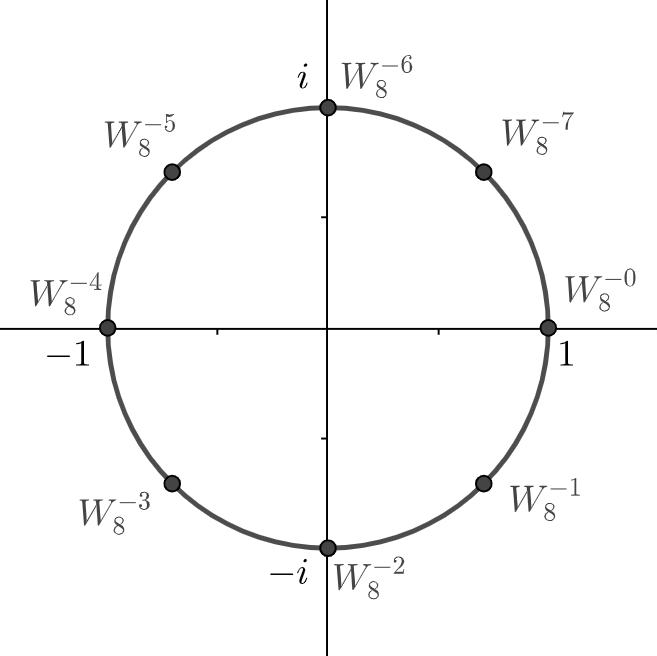
\includegraphics[height=6cm]{./assets/unitCircle.png}
		\caption{Une seule somme}
		\label{fig:split}
	\end{minipage}
	\hfill
	\begin{minipage}{0.5\textwidth}
		\centering
		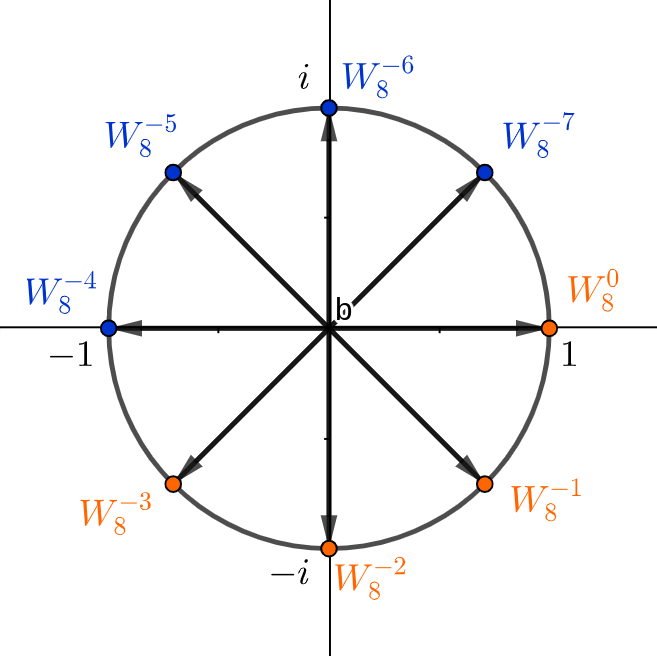
\includegraphics[height=6cm]{./assets/unitCircleSplit.png}
		\caption{Après la division en 2 sommes}
		\label{fig:split2}
	\end{minipage}
\end{figure}

\noindent En orange, les termes $G_{k}$, et en bleu les termes $G_{k+N/2}$. Une symétrie centrale apparaît, il est alors clair que l'on a besoin de calculer seulement les termes oranges pour trouver les termes bleus. L'un étant l'opposé de l'autre. On passe du calcul de 8 à 4 termes! Nous l'avions déjà montré par le calcul, de l'équation (15) à (20). Cela nous permet de déduire une nouvelle propriété des racines n-ième de l'unité (seulement si n est pair) : 

\begin{equation}
	-\krootofunity{k}{n} = \krootofunity{k+n/2}{n}
\end{equation}

\subsubsection{Papillon}

Il est très commun de sereprésenter la transformée de Fourier par un diagramme nommé papillon (\textit{butterfly}) - Il montre comment se combinent les termes avec les racines n-ième de l'unité. Profitons en pour montrer comment se décompose un signal. 
\\~~~
\noindent Exemple avec un vecteur de taille N = 8 :
\newpage \noindent On commence par décomposer le vecteur original en vecteurs de taille 1 à l'aide des divisions successives par 2. Ainsi on peut calculer la transformée de Fourier de chacun d'entre eux très simplement!
\begin{figure}[!htb]
	\centering
	\includegraphics[height=7cm]{./assets/divide.png}
	\caption{Divide . . .}
	\label{fig:divide}
\end{figure}

\noindent Puis on recompose les 16 vecteurs de taille 1 en 8 vecteurs de taille 2, puis 4 vecteurs de taille 4, puis 2 vecteurs de taille 8, puis enfin notre vecteur résultat de taille 16! Le fameux diagramme papillon - On peut d'ailleurs voir qu'on utilise seulement les \textbf{k/2 racines n-ièmes de l'unité} à chaque étape.

\begin{figure}[!htb]
	\centering
	\includegraphics[height=9cm]{./assets/conquer.png}
	\caption{. . . and Conquer!}
	\label{fig:conquer}
\end{figure}

\noindent Le vecteur obtenu en sortie est le signal transformé.\textit{ De la même manière que pour la transformée brute, il suffira de changer un signe - par un signe + dans nos exponentielles pour obtenir la transformée inverse : Cela correspond à passer de $\bm{\krootofunity{-k}{n}}$ à $\bm{\krootofunity{k}{n}}$}

\end{document}
